\documentclass[conference]{IEEEtran}
\IEEEoverridecommandlockouts

\usepackage{cite}
\usepackage{amsmath,amssymb,amsfonts}
\usepackage{algorithm}
\usepackage{algorithmic}
\usepackage{graphicx}
\usepackage{textcomp}
\usepackage{xcolor}
\def\BibTeX{{\rm B\kern-.05em{\sc i\kern-.025em b}\kern-.08em
    T\kern-.1667em\lower.7ex\hbox{E}\kern-.125emX}}

\begin{document}

\title{Three-Dimensional Voronoi Adaptive Coverage and Dynamic Boundary Tracking for Underwater Oil Spill Monitoring}

\author{\IEEEauthorblockN{huataojia}
\IEEEauthorblockA{\textit{Affiliation}\\
City, Country\\
email@example.com}}
% \author{\IEEEauthorblockN{Xiaofeng Zong}
% \IEEEauthorblockA{\textit{Affiliation}\\
% City, Country\\
% email@example.com}}
% \author{\IEEEauthorblockN{Haochao Lin}
% \IEEEauthorblockA{\textit{Affiliation}\\
% City, Country\\
% email@example.com}}
\maketitle

\begin{abstract}
Underwater oil leakage creates time-varying three-dimensional plumes that challenge multi-AUV monitoring under limited sensing ranges. Standard density-weighted CVT can cause cluster collapse, drawing vehicles toward the concentration peak and weakening boundary coverage. This paper proposes CVT-DBT, combining three-dimensional Voronoi adaptive coverage with dynamic boundary tracking. The method uses a continuous-release plume model, volume-based Voronoi partitioning, and a velocity-constrained controller with centroid feedback, feedforward, boundary tracking, and dispersion. Simulations improve final coverage from 38.24\% to 58.86\% and reduce boundary RMSE from 66.75 m to 15.94 m, while satisfying AUV speed limits.
\end{abstract}

\begin{IEEEkeywords}
Underwater oil spill monitoring, multi-AUV cooperation, three-dimensional Voronoi coverage, dynamic boundary tracking, continuous-release plume, cluster collapse.
\end{IEEEkeywords}

\section{Introduction}
Underwater oil spills pose major risks to marine environmental safety and offshore engineering operations. Unlike surface spills, underwater leakage forms time-varying three-dimensional pollution plumes under ocean-current transport, turbulent diffusion, buoyancy-driven rise, and natural decay. The migration and diffusion of underwater oil spills are strongly affected by leakage rate and ocean-current velocity \cite{zhang2020oil}. Practical oil spill models must therefore account for transport, diffusion, decay, and boundary effects \cite{fingas2022overview}.

Autonomous underwater vehicles (AUVs) are well suited to underwater pollution monitoring because they provide autonomous mobility, three-dimensional maneuverability, and close-range sensing. A key challenge in multi-AUV monitoring is to adjust vehicle distributions as the pollution field evolves. Effective monitoring must cover both high-concentration regions and the outer plume boundary. Classical coverage control is usually formulated with Voronoi partitions and locational cost functions \cite{cortes2004coverage}. Lloyd-type iterations and centroid feedback then provide numerical mechanisms for approaching centroidal Voronoi configurations \cite{du2006lloyd}.

However, standard centroidal Voronoi tessellation (CVT) methods are not sufficient for underwater oil spill monitoring. Because the concentration peak is usually near the leakage source, pure density-weighted centroid feedback attracts AUVs toward the high-concentration core. This behavior can reduce the locational cost, but it weakens monitoring of the expanding outer boundary. In this paper, this behavior is referred to as cluster collapse.

To address this limitation, this paper proposes a three-dimensional Voronoi adaptive coverage and dynamic boundary tracking method for multi-AUV underwater oil spill monitoring. The main contributions are as follows:
\begin{itemize}
\item A continuous-release three-dimensional advection--diffusion--decay plume model is developed through temporal convolution of historically released oil parcels.
\item A volume-based three-dimensional Voronoi coverage model is formulated, in which AUVs move within the underwater domain rather than on a two-dimensional surface.
\item A dynamic boundary sampling and spatially balanced assignment mechanism is introduced, yielding a CVT-DBT control law with centroid feedback, feedforward compensation, boundary tracking, and dispersion terms.
\item Comparative simulations with standard CVT and three-dimensional lawnmower coverage show the advantages of the proposed method in dynamic coverage ratio, boundary tracking RMSE, and velocity-constrained feasibility.
\end{itemize}

\section{Related Work}
\subsection{Multi-Agent Voronoi Coverage Control}
Multi-agent coverage control coordinates multiple mobile sensors or robots to monitor a target domain effectively. Cortes et al. established a fundamental coverage control framework based on Voronoi partitions and locational cost functions \cite{cortes2004coverage}. In this framework, each agent is assigned the region closest to itself and moves toward the density-weighted centroid of its Voronoi cell.

Centroidal Voronoi tessellation and Lloyd algorithms provide important computational foundations for coverage control. Du et al. studied the convergence of Lloyd algorithms for computing centroidal Voronoi tessellations \cite{du2006lloyd}. However, conventional CVT methods are mainly designed for static or slowly varying density fields. When the density field is highly nonuniform, agents tend to concentrate around high-density regions. This behavior can cause insufficient boundary monitoring in oil spill scenarios.

\subsection{Time-Varying Density Coverage Control}
In practical environmental monitoring, the density function is often time varying. Pierson et al. studied generalized coverage control for time-varying density functions \cite{pierson2019generalized}. These studies indicate that pure feedback to the instantaneous centroid may be insufficient in dynamic environments. Feedforward or prediction mechanisms can improve tracking performance. Unlike general time-varying coverage, underwater oil spill monitoring requires both coverage of high-concentration regions and persistent tracking of the expanding outer boundary.

\subsection{Underwater Oil Spill Modeling}
Underwater oil spill migration and diffusion are affected by leakage rate, ocean-current velocity, turbulent diffusion, buoyancy, and natural decay. Previous studies have analyzed how leakage rate and ocean-current velocity affect underwater spill migration \cite{zhang2020oil}. Fingas reviewed oil spill modeling and simulation for both surface and subsurface applications \cite{fingas2022overview}. Motivated by these physical insights, this paper develops a continuous-release three-dimensional plume model and couples it with multi-AUV coverage control.

\section{Problem Formulation}
Let the three-dimensional monitoring domain be
\begin{equation}
\Omega=[x_{\min},x_{\max}]\times[y_{\min},y_{\max}]\times[z_{\min},z_{\max}]\subset\mathbb{R}^3,
\end{equation}
where $z=0$ denotes the sea surface and $z<0$ denotes the underwater region. A spatial point is denoted by
\begin{equation}
q=[x,y,z]^T\in\Omega,\quad dq=dxdydz.
\end{equation}

Consider $n$ AUVs with positions
\begin{equation}
p_i(t)=[x_i(t),y_i(t),z_i(t)]^T\in\Omega,\quad i=1,\ldots,n.
\end{equation}
Each AUV satisfies the velocity constraint
\begin{equation}
\|\dot p_i(t)\|\leq v_{\max}.
\end{equation}

Given the AUV position set $P(t)=\{p_1(t),\ldots,p_n(t)\}$, the three-dimensional Voronoi cell of the $i$-th AUV is defined as
\begin{equation}
V_i(t)=\{q\in\Omega\mid \|q-p_i(t)\|\leq \|q-p_j(t)\|,\forall j\neq i\}.
\end{equation}
Thus, $V_i(t)$ is a volume region rather than a two-dimensional plane or surface.

This partition follows directly from the locational coverage objective. For any spatial point $q\in\Omega$, the local sensing cost contributed by the $i$-th AUV is proportional to $\|q-p_i(t)\|^2$. Assigning $q$ to the nearest AUV minimizes this local term pointwise. This yields the nearest-neighbor partition in the three-dimensional Euclidean domain. Therefore, the global coverage cost can be decomposed over three-dimensional Voronoi volume cells rather than over a planar projection or plume surface.

Let $C(q,t)$ denote the oil concentration field. The coverage density function is defined as
\begin{equation}
\phi(q,t)=\alpha C_{\mathrm{norm}}(q,t)+\beta,
\end{equation}
where
\begin{equation}
C_{\mathrm{norm}}(q,t)=\min\left(\frac{C(q,t)}{C_{\max}^{\mathrm{est}}},1\right).
\end{equation}

The density-weighted load of the $i$-th Voronoi cell is
\begin{equation}
M_i(t)=\int_{V_i(t)}\phi(q,t)dq,
\end{equation}
and the corresponding density-weighted centroid is
\begin{equation}
c_i(t)=
\frac{\int_{V_i(t)}q\phi(q,t)dq}
{\int_{V_i(t)}\phi(q,t)dq}.
\end{equation}

The locational coverage cost is defined as
\begin{equation}
\mathcal{H}(P,t)=
\sum_{i=1}^{n}
\int_{V_i(t)}
\phi(q,t)\|q-p_i(t)\|^2dq.
\end{equation}
For fixed Voronoi cells and a frozen density field, differentiating the $i$-th cell cost with respect to $p_i$ gives
\begin{equation}
\frac{\partial}{\partial p_i}
\int_{V_i(t)}
\phi(q,t)\|q-p_i(t)\|^2dq
=2M_i(t)(p_i(t)-c_i(t)).
\end{equation}
Hence, the stationary condition is $p_i(t)=c_i(t)$, which motivates the centroid-seeking update used in CVT-based coverage control.

\section{Continuous-Release Three-Dimensional Oil Plume Model}
Let the leakage source be located at $q_s=[x_s,y_s,z_s]^T$, where $z_s<0$. The concentration field $C(q,t)$ satisfies the three-dimensional advection--diffusion--decay equation:
\begin{equation}
\begin{aligned}
\frac{\partial C}{\partial t}
&+u\frac{\partial C}{\partial x}
+w_b\frac{\partial C}{\partial z} \\
&=
D_x\frac{\partial^2 C}{\partial x^2}
+D_y\frac{\partial^2 C}{\partial y^2}
+D_z\frac{\partial^2 C}{\partial z^2}
-\lambda C
+Q\delta(q-q_s).
\end{aligned}
\end{equation}

A continuous leakage process is represented as a temporal convolution of historically released oil parcels. Let $\tau$ be the release time and
\begin{equation}
a=t-\tau
\end{equation}
be the age of the released parcel. The center of the parcel evolves as
\begin{equation}
x_c(a)=x_s+ua,\quad y_c(a)=y_s,\quad z_c(a)=\min(0,z_s+w_ba).
\end{equation}
The diffusion scales are
\begin{equation}
\sigma_k(a)=\sqrt{\sigma_{k0}^2+2D_ka},\quad k\in\{x,y,z\}.
\end{equation}
The nonzero initial diffusion scale $\sigma_{k0}>0$ regularizes the point-source model and avoids a concentration singularity.

The concentration field is approximated by
\begin{equation}
\begin{aligned}
C(q,t)=\int_0^t
&\frac{Qe^{-\lambda a}}
{(2\pi)^{3/2}\sigma_x(a)\sigma_y(a)\sigma_z(a)} \\
&\times
\exp\left[-\frac{(x-x_c(a))^2}{2\sigma_x^2(a)}\right] \\
&\times
\exp\left[-\frac{(y-y_c(a))^2}{2\sigma_y^2(a)}\right]
\Gamma_z(z,a)d\tau,
\end{aligned}
\end{equation}
where
\begin{equation}
\begin{aligned}
\Gamma_z(z,a)=
&\exp\left[-\frac{(z-z_c(a))^2}{2\sigma_z^2(a)}\right] \\
&+
\exp\left[-\frac{(z+z_c(a))^2}{2\sigma_z^2(a)}\right].
\end{aligned}
\end{equation}
The second term is an image term with respect to the sea surface. It approximately satisfies the zero-flux boundary condition at $z=0$. Seabed reflection is neglected by assuming that the source is sufficiently above the seabed and that the main plume body does not reach the seabed during the monitoring window.

If AUV monitoring starts after a pre-leakage duration $t_0$, the physical time used in the plume model is
\begin{equation}
t=t_0+t_m,
\end{equation}
where $t_m$ is the monitoring time.

The dynamic plume boundary is defined as the concentration isosurface
\begin{equation}
\partial\mathcal{P}(t)=
\{q\in\Omega\mid C(q,t)=\eta C_{\max}(t)\}.
\end{equation}

\section{Three-Dimensional Voronoi Adaptive Coverage and Dynamic Boundary Tracking}
At each time instant, the three-dimensional Voronoi partition and density-weighted centroids are computed from the current concentration field. To prevent cluster collapse, the proposed method also samples and assigns the dynamic plume boundary in three-dimensional space.

Let the sampled boundary point set be
\begin{equation}
\mathcal{B}(t)=\{b_1(t),\ldots,b_m(t)\},\quad b_l(t)\in\partial\mathcal{P}(t).
\end{equation}
With the plume center $q_c(t)$ as the reference point, define
\begin{equation}
r_l(t)=b_l(t)-q_c(t),
\end{equation}
and the corresponding unit direction
\begin{equation}
s_l(t)=\frac{r_l(t)}{\|r_l(t)\|}.
\end{equation}

The boundary surface is approximately partitioned into balanced three-dimensional solid-angle sectors. The boundary subset assigned to the $i$-th AUV satisfies
\begin{equation}
\mathcal{B}_i(t)\subset\mathcal{B}(t),\quad
\bigcup_{i=1}^{n}\mathcal{B}_i(t)=\mathcal{B}(t),\quad
\mathcal{B}_i(t)\cap\mathcal{B}_j(t)=\emptyset.
\end{equation}

The boundary tracking target is
\begin{equation}
b_i^{\ast}(t)=
\begin{cases}
\frac{1}{N_i(t)}\sum_{b_l(t)\in\mathcal{B}_i(t)}b_l(t), & N_i(t)>0,\\
p_i(t), & N_i(t)=0,
\end{cases}
\end{equation}
where $N_i(t)=\operatorname{card}(\mathcal{B}_i(t))$.

The nominal CVT-DBT velocity command is
\begin{equation}
\begin{aligned}
v_i^{\mathrm{nom}}(t)
={}&k_c(c_i(t)-p_i(t))
+\gamma_{\mathrm{ff}}\dot c_i(t) \\
&+k_b(b_i^{\ast}(t)-p_i(t))
+v_{\mathrm{sep},i}(t).
\end{aligned}
\end{equation}
The centroid velocity is approximated by
\begin{equation}
\dot c_i(t)\approx
\frac{c_i(t)-c_i(t-\Delta t)}{\Delta t}.
\end{equation}
The dispersion term is
\begin{equation}
v_{\mathrm{sep},i}(t)
=
\sum_{j\neq i}
\rho_{ij}(t)
\frac{p_i(t)-p_j(t)}
{\|p_i(t)-p_j(t)\|}.
\end{equation}

The actual control velocity is obtained by
\begin{equation}
v_i(t)=\operatorname{sat}_{v_{\max}}(v_i^{\mathrm{nom}}(t)),
\end{equation}
where
\begin{equation}
\operatorname{sat}_{v_{\max}}(v)=
\begin{cases}
v, & \|v\|\leq v_{\max},\\
v_{\max}\frac{v}{\|v\|}, & \|v\|>v_{\max}.
\end{cases}
\end{equation}
The position update is
\begin{equation}
p_i(t+\Delta t)=p_i(t)+v_i(t)\Delta t.
\end{equation}

Algorithm \ref{alg:cvt_dbt} summarizes one discrete CVT-DBT iteration used in the simulations. The three-dimensional Voronoi integrals are approximated by mixed uniform and plume-biased importance samples. Each sample is assigned to its nearest AUV. This implementation is consistent with the volume Voronoi definition while avoiding explicit construction of clipped three-dimensional Voronoi polyhedra.

\begin{algorithm}[t]
\caption{CVT-DBT Iteration for Dynamic Underwater Oil Plume Monitoring}
\label{alg:cvt_dbt}
\begin{algorithmic}[1]
\REQUIRE AUV positions $P(t)$, previous centroids $C_{\mathrm{prev}}$, plume parameters, $\Delta t$, gains $k_c$, $\gamma_{\mathrm{ff}}$, $k_b$, and $v_{\max}$
\ENSURE Updated positions $P(t+\Delta t)$, current centroids $C(t)$, and boundary targets $B^{\ast}(t)$
\STATE Draw mixed uniform and plume-biased samples in $\Omega$.
\STATE Evaluate $\phi(q,t)$ and the importance weights at all samples.
\STATE Assign each sample to the nearest AUV to approximate $V_i(t)$.
\STATE Compute density-weighted centroids $c_i(t)$ for all AUVs.
\IF{$C_{\mathrm{prev}}$ is available}
\STATE Approximate $\dot c_i(t)\leftarrow(c_i(t)-c_{i,\mathrm{prev}})/\Delta t$.
\ELSE
\STATE Set $\dot c_i(t)\leftarrow0$.
\ENDIF
\STATE Sample boundary candidates near $C(q,t)=\eta C_{\max}(t)$.
\STATE Assign boundary samples to AUVs by balanced angular sectors around the plume center.
\STATE Compute $b_i^{\ast}(t)$ as the mean assigned boundary point; use $p_i(t)$ if no point is assigned.
\STATE Construct $v_i^{\mathrm{nom}}$ using centroid feedback, centroid-velocity feedforward, boundary tracking, and dispersion.
\STATE Saturate $v_i^{\mathrm{nom}}$ by $v_{\max}$ to obtain $v_i(t)$.
\STATE Update $p_i(t+\Delta t)\leftarrow p_i(t)+v_i(t)\Delta t$ and project it into $\Omega$.
\end{algorithmic}
\end{algorithm}

Let $N_s$ be the number of centroid samples, $N_b$ the number of boundary samples, $n$ the number of AUVs, and $L$ the number of temporal convolution substeps for plume evaluation. The dominant per-step cost is approximately $O(N_s n+N_sL+N_bL+n^2)$. The four terms correspond to nearest-agent assignment, density evaluation at centroid samples, boundary concentration evaluation, and pairwise dispersion, respectively. In the considered experiments, $n=8$, so the main computational burden comes from sampling-based density and boundary evaluation.

\subsection{Theoretical Property and Stability Discussion}
For a static density field, or within a single control step where $\phi(q,t)$ is treated as frozen, standard CVT centroid feedback has a Lyapunov-like descent property. Consider the frozen locational cost
\begin{equation}
\mathcal{H}(P)=
\sum_{i=1}^{n}
\int_{V_i}
\phi(q)\|q-p_i\|^2dq.
\end{equation}
For nondegenerate Voronoi cells with
\begin{equation}
M_i=\int_{V_i}\phi(q)dq>0,
\end{equation}
the classical CVT first variation gives
\begin{equation}
\frac{\partial \mathcal{H}}{\partial p_i}
=2M_i(p_i-c_i),
\end{equation}
where the boundary terms induced by the Voronoi partition cancel between adjacent cells. Under the standard centroid feedback
\begin{equation}
\dot p_i=-k_c(p_i-c_i),\quad k_c>0,
\end{equation}
the derivative of $\mathcal{H}$ along the closed-loop trajectory satisfies
\begin{equation}
\begin{aligned}
\dot{\mathcal{H}}
&=
\sum_{i=1}^{n}
\left(\frac{\partial \mathcal{H}}{\partial p_i}\right)^T\dot p_i \\
&=-2k_c\sum_{i=1}^{n}M_i\|p_i-c_i\|^2\leq0.
\end{aligned}
\end{equation}
Therefore, in the fixed-density case, the locational cost is nonincreasing. By LaSalle's invariance principle, the standard CVT dynamics converge to the invariant set satisfying $p_i=c_i$. This set corresponds to a local centroidal Voronoi configuration.

The proposed CVT-DBT law is not a pure gradient descent of $\mathcal{H}(P,t)$. The centroid feedback term inherits the local descent tendency described above. The centroid-velocity feedforward, boundary tracking, dispersion, and velocity saturation terms are introduced for dynamic plume monitoring and actuator feasibility. Therefore, the complete time-varying CVT-DBT system should not be claimed to converge globally and asymptotically to the minimizer of $\mathcal{H}(P,t)$. Instead, it deliberately trades part of locational-cost optimality for boundary tracking accuracy. This tradeoff is consistent with the simulation results: standard CVT attains a lower final $\mathcal{H}$ but suffers from cluster collapse, whereas CVT-DBT achieves a higher dynamic coverage ratio and a much smaller boundary RMSE.

\section{Simulation Results and Analysis}
\subsection{Simulation Setup}
The simulations are conducted in MATLAB 2024b. The main parameters are listed in Table \ref{tab:params}.

\begin{table}[htbp]
\caption{Simulation Parameters}
\label{tab:params}
\begin{center}
\begin{tabular}{|c|c|c|}
\hline
\textbf{Parameter} & \textbf{Value} & \textbf{Description}\\
\hline
Number of AUVs & 8 & Cooperative monitoring\\
\hline
Source position & $[150,0,-180]$ m & Underwater source\\
\hline
Current velocity & $0.50$ m/s & Positive $x$ direction\\
\hline
Buoyancy velocity & $0.22$ m/s & Positive $z$ direction\\
\hline
Pre-leakage time & $80$ s & Initial plume exists\\
\hline
Simulation steps & 200 & 1 s per step\\
\hline
Sensing radius & 50 m & AUV sensing range\\
\hline
Maximum speed & 3.5 m/s & Velocity constraint\\
\hline
Boundary threshold & $3.5\%C_{\max}$ & Plume boundary\\
\hline
\end{tabular}
\end{center}
\end{table}

Three methods are compared: Proposed CVT-DBT, Standard CVT, and Lawnmower CPP. The standard CVT method uses only centroid feedback,
\begin{equation}
v_i(t)=k_c(c_i(t)-p_i(t)).
\end{equation}
The lawnmower method follows a preplanned three-dimensional scanning path and does not adapt to the real-time plume state.

\subsection{Evaluation Metrics}
The coverage quality is
\begin{equation}
\mathcal{H}(P,t)=
\int_{\Omega}\phi(q,t)\min_i\|q-p_i(t)\|^2dq.
\end{equation}
The dynamic coverage ratio is
\begin{equation}
CR(t)=
\frac{
\int_{\mathcal{P}(t)}
\mathbf{1}\left(\min_i\|q-p_i(t)\|\leq R_s\right)dq
}{
\int_{\mathcal{P}(t)}dq
}.
\end{equation}
The boundary tracking RMSE is
\begin{equation}
RMSE(t)=
\sqrt{
\frac{1}{n}
\sum_{i=1}^{n}
\min_{b_l(t)\in\mathcal{B}(t)}
\|p_i(t)-b_l(t)\|^2
}.
\end{equation}
The AUV speed is
\begin{equation}
v_i^{\mathrm{speed}}(t)=
\frac{\|p_i(t+\Delta t)-p_i(t)\|}{\Delta t}.
\end{equation}

\subsection{Results}
Fig. \ref{fig:plume} shows the three-dimensional plume isosurfaces and AUV trajectories. The proposed method distributes AUVs between the high-concentration core and the outer boundary. As a result, the vehicles form a spatial envelope around the plume.

\begin{figure}[htbp]
\centerline{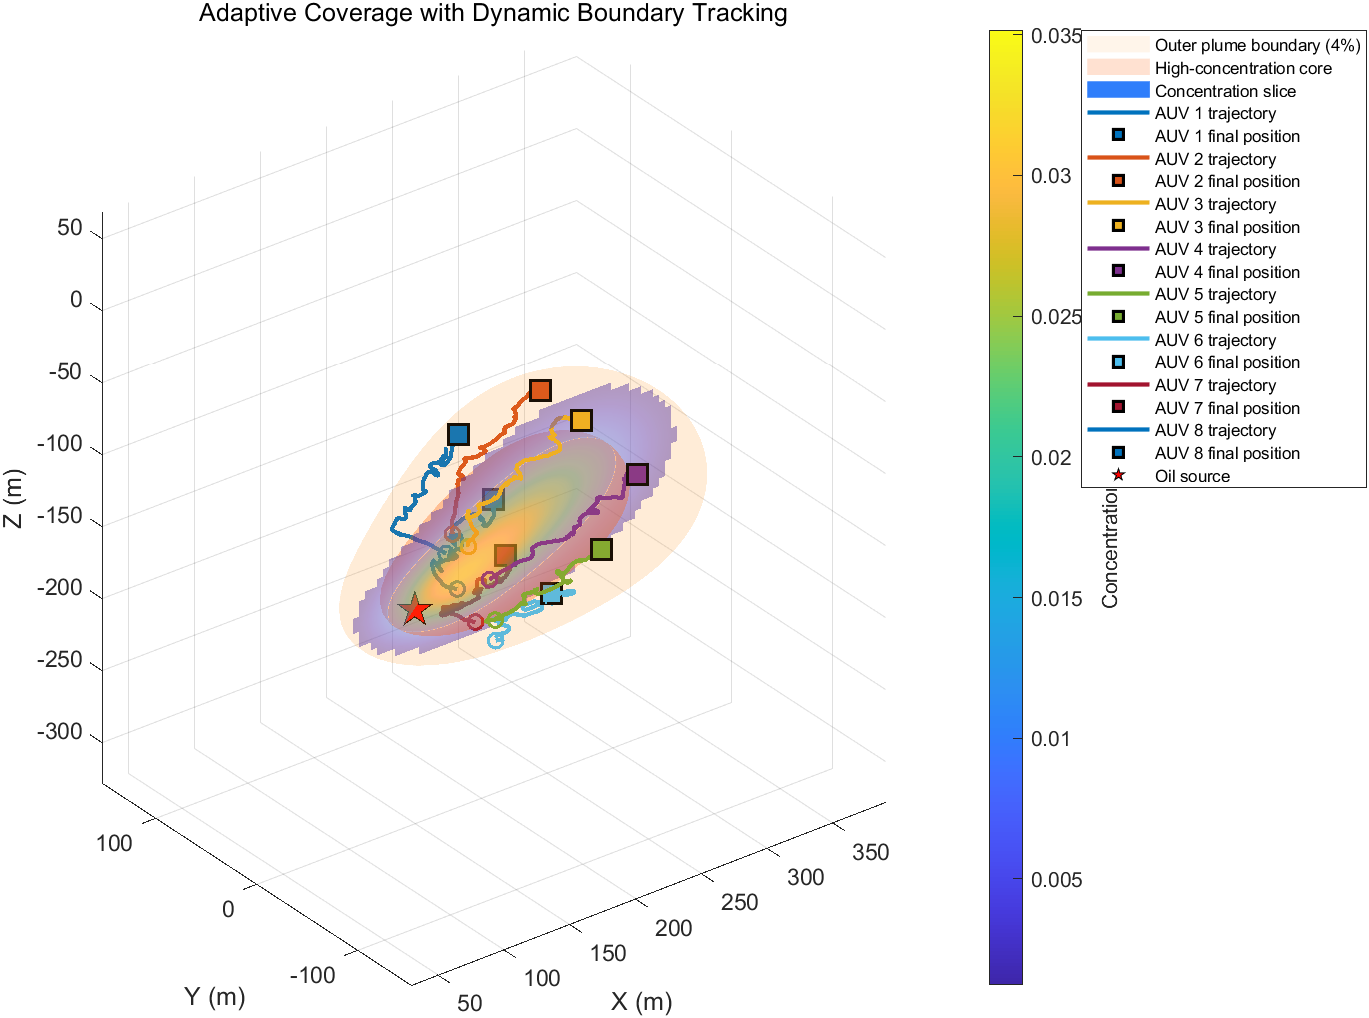
\includegraphics[width=\linewidth]{figures/step8_plume_agents_tracking.png}}
\caption{Three-dimensional oil plume and AUV trajectories.}
\label{fig:plume}
\end{figure}

Fig. \ref{fig:voronoi} shows the three-dimensional Voronoi regions. The result confirms that the responsibility domains are volume regions rather than two-dimensional surfaces.

\begin{figure}[htbp]
\centerline{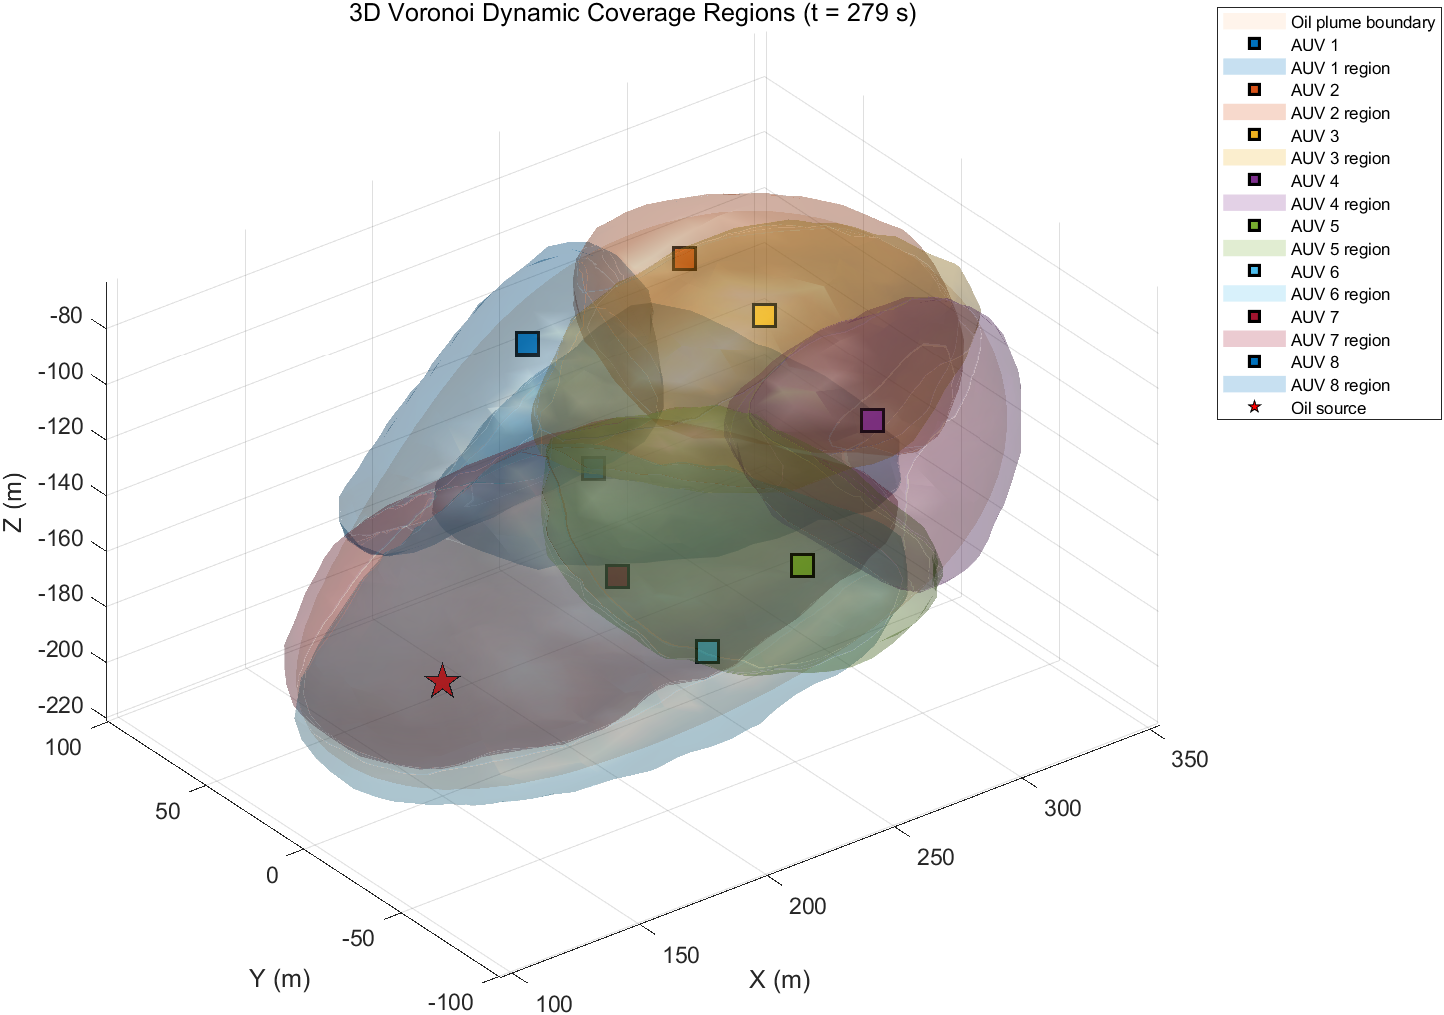
\includegraphics[width=\linewidth]{figures/step8_voronoi_3d.png}}
\caption{Three-dimensional Voronoi coverage regions.}
\label{fig:voronoi}
\end{figure}

A Voronoi responsibility region specifies which AUV is responsible for a spatial location. It is not equivalent to the plume volume actually sensed within the finite sonar radius. To link the metric definition with visual evidence, Fig. \ref{fig:coverage_regions} shows the actual sensing coverage at the final time. The translucent spheres denote sensing ranges with $R_s=50$ m. Green samples denote plume volume covered by at least one AUV, and gray samples denote uncovered plume volume. This figure directly corresponds to the definition of $CR(T)$. The dynamic coverage ratio measures the fraction of plume volume within at least one AUV sensing radius, not the fraction assigned by Voronoi responsibility regions.

\begin{figure}[htbp]
\centerline{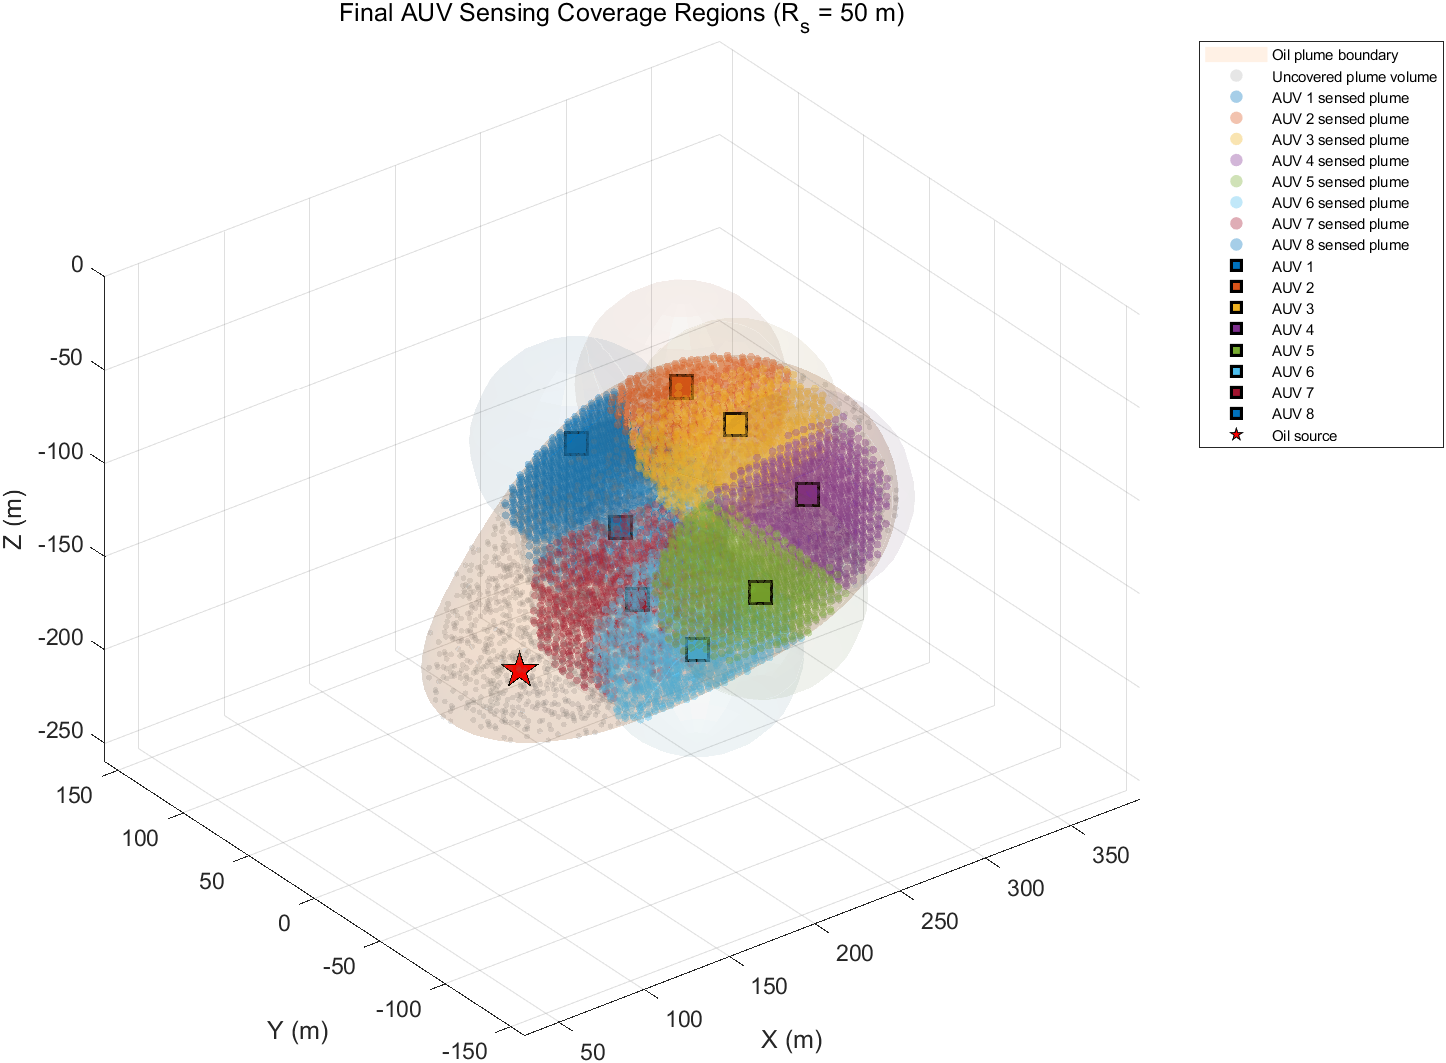
\includegraphics[width=\linewidth]{figures/step8_coverage_regions_3d.png}}
\caption{Actual sensing coverage region at the final time.}
\label{fig:coverage_regions}
\end{figure}

Fig. \ref{fig:H} compares the coverage quality. Standard CVT achieves a lower final coverage cost because the AUVs collapse toward the high-concentration core. However, this behavior sacrifices boundary monitoring.

\begin{figure}[htbp]
\centerline{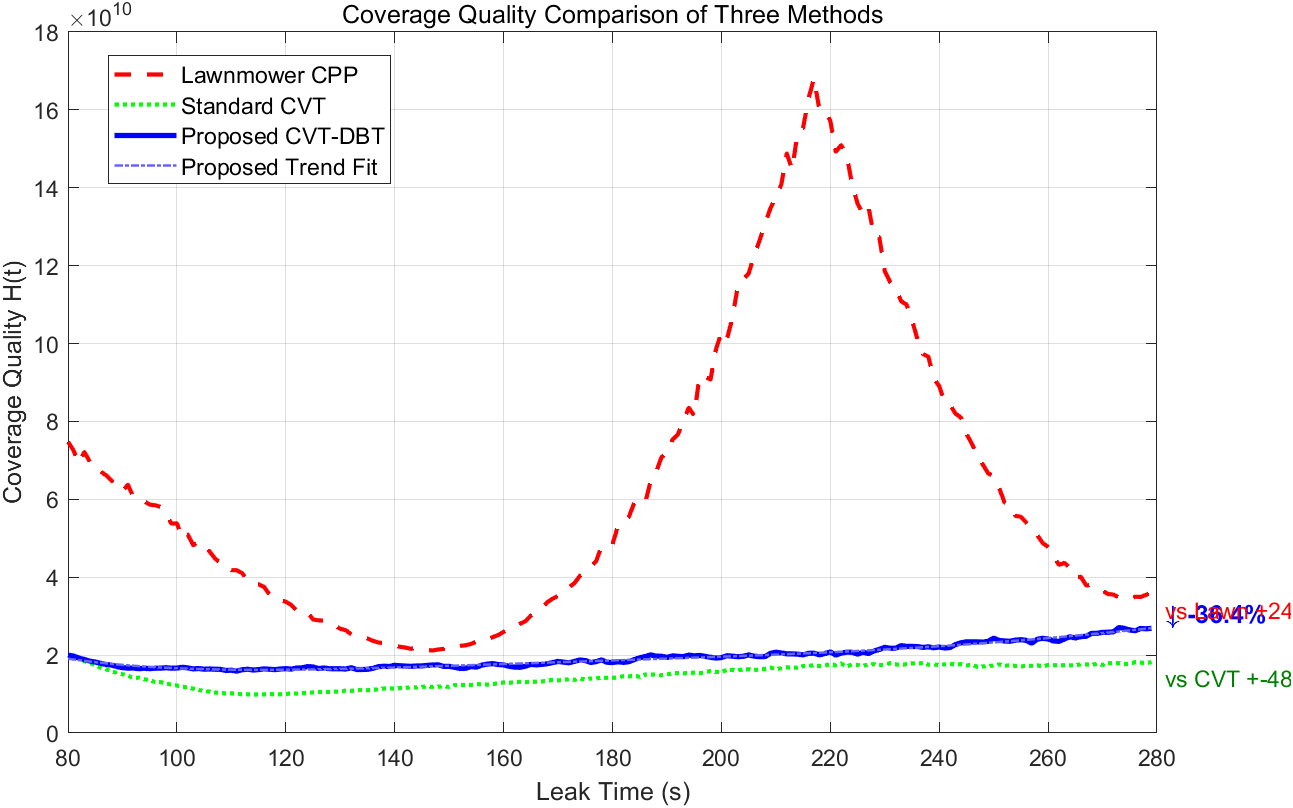
\includegraphics[width=\linewidth]{figures/step8_coverage_quality.png}}
\caption{Comparison of coverage quality.}
\label{fig:H}
\end{figure}

Fig. \ref{fig:metrics} shows the dynamic coverage ratio and boundary tracking RMSE. The key metrics are listed in Table \ref{tab:results}.

\begin{figure}[htbp]
\centerline{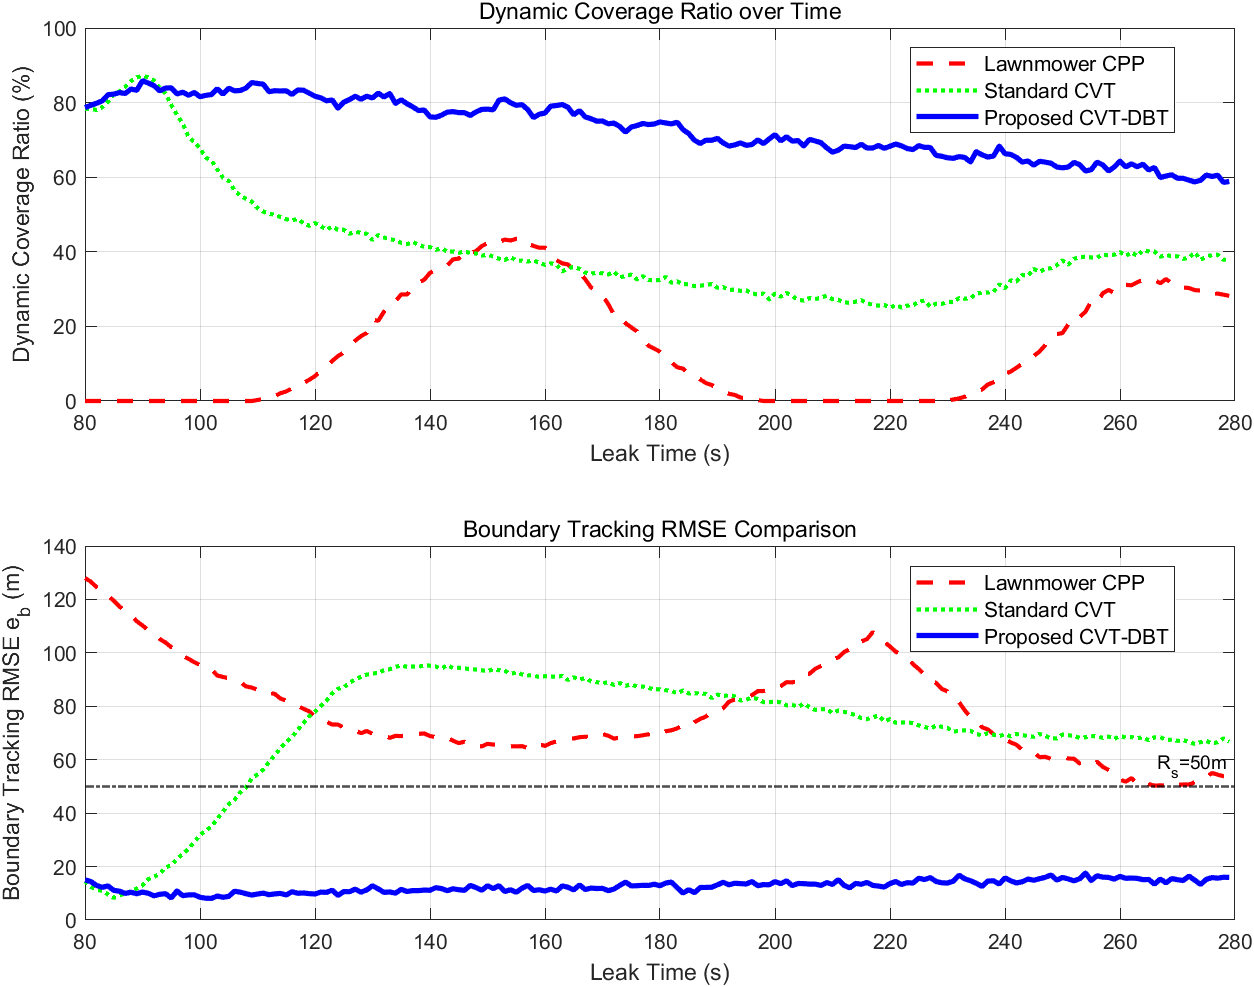
\includegraphics[width=\linewidth]{figures/step8_coverage_metrics.png}}
\caption{Dynamic coverage ratio and boundary tracking RMSE.}
\label{fig:metrics}
\end{figure}

\begin{table}[htbp]
\caption{Comparison of Key Metrics}
\label{tab:results}
\begin{center}
\begin{tabular}{|c|c|c|c|}
\hline
\textbf{Method} & \textbf{$\mathcal{H}(T)$} & \textbf{$CR(T)$} & \textbf{RMSE}\\
\hline
CVT-DBT & $2.687\times10^{10}$ & 58.86\% & 15.94 m\\
\hline
Standard CVT & $1.821\times10^{10}$ & 38.24\% & 66.75 m\\
\hline
Lawnmower CPP & $3.606\times10^{10}$ & 28.20\% & 54.10 m\\
\hline
\end{tabular}
\end{center}
\end{table}

Compared with standard CVT, the proposed method reduces the boundary RMSE from 66.75 m to 15.94 m. This corresponds to an approximately 76.1\% reduction and a 4.2-fold improvement in boundary tracking accuracy. The dynamic coverage ratio also increases from 38.24\% to 58.86\%, and the mean ratio over the last 20 steps reaches 60.88\%. Together with Fig. \ref{fig:coverage_regions}, these results show that CVT-DBT does not merely improve $CR(T)$ numerically. Under the finite sensing radius constraint, it distributes AUVs between the plume core and the spreading boundary. The actually sensed volume therefore forms a continuous three-dimensional monitoring envelope. Dynamic boundary tracking and spatially balanced assignment effectively mitigate cluster collapse.

Fig. \ref{fig:control} shows the AUV speed curves. All AUV speeds are limited by the saturation constraint $v_{\max}=3.5$ m/s. The maximum recorded speed is 3.50 m/s, and the average speed is approximately 3.47 m/s. The smooth curves indicate that the control inputs are practically feasible.

\begin{figure}[htbp]
\centerline{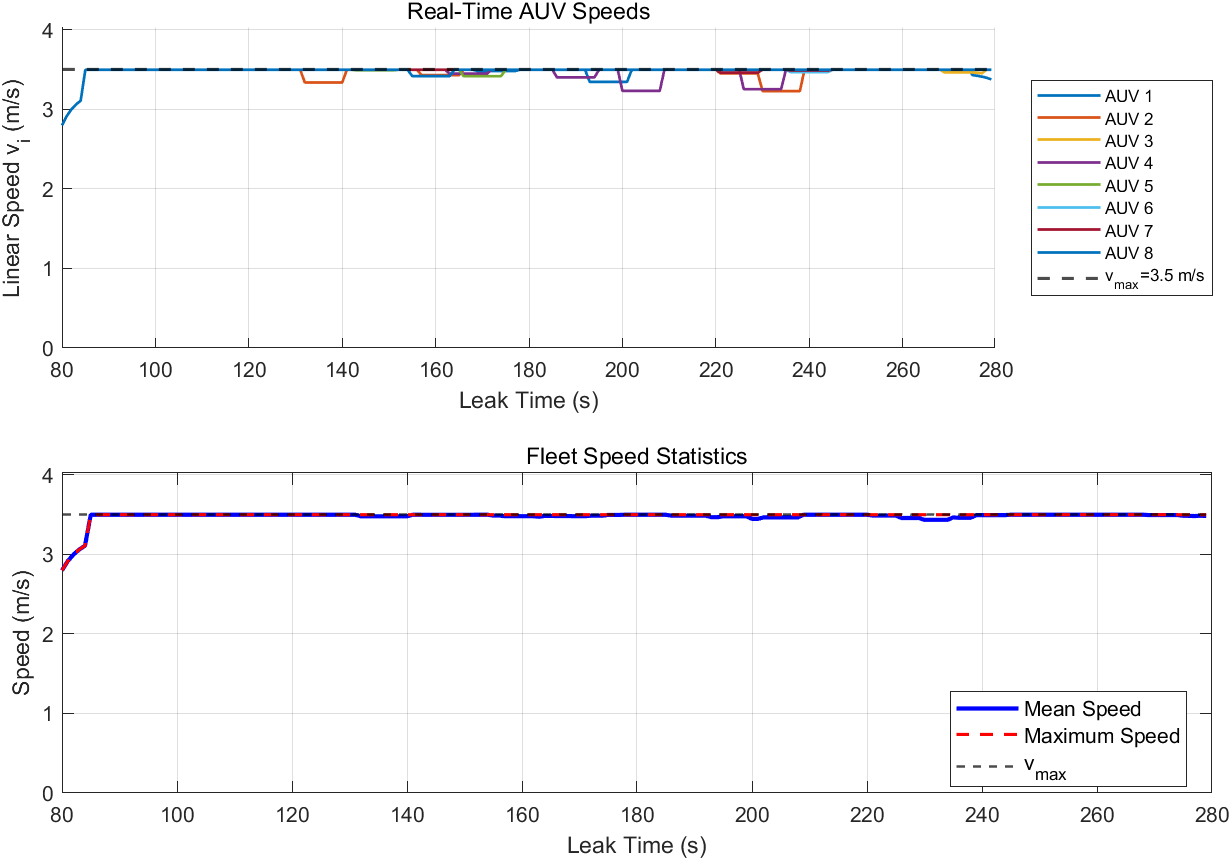
\includegraphics[width=\linewidth]{figures/step8_control_input.png}}
\caption{AUV control input speed curves.}
\label{fig:control}
\end{figure}

\section{Conclusion}
This paper proposed a multi-AUV cooperative monitoring method that integrates three-dimensional Voronoi adaptive coverage with dynamic boundary tracking for continuous underwater oil spill monitoring. A continuous-release three-dimensional plume model was developed by considering ocean-current transport, anisotropic diffusion, buoyancy-driven rise, and natural decay. A volume-based Voronoi partition and density-weighted centroid were then constructed to guide AUVs toward high-risk regions. To address cluster collapse, dynamic boundary sampling and spatially balanced assignment were introduced. These components yield a velocity-constrained control law with centroid feedback, centroid-velocity feedforward, boundary tracking, and dispersion terms.

Simulation results show that standard CVT achieves a lower locational cost but suffers from cluster collapse. Its final dynamic coverage ratio is 38.24\%, and its boundary RMSE is 66.75 m. In contrast, the proposed CVT-DBT method increases the dynamic coverage ratio to 58.86\%, reaches a last-20-step mean coverage ratio of 60.88\%, and reduces the boundary RMSE to 15.94 m while satisfying the AUV velocity constraint. The actual sensing coverage visualization further confirms that the reported dynamic coverage comes from plume volume covered within finite sonar ranges. It is not obtained by treating Voronoi responsibility regions as monitored regions. This closes the logical chain from plume model and control law to evaluation metrics and visual validation. Future work will consider collision avoidance, communication constraints, complex seabed geometry, and control-barrier-function-based safety filtering.

\begin{thebibliography}{00}

\bibitem{cortes2004coverage}
J. Cortés, S. Martínez, T. Karatas, and F. Bullo, ``Coverage control for mobile sensing networks,'' \textit{IEEE Transactions on Robotics and Automation}, vol. 20, no. 2, pp. 243--255, 2004, doi: 10.1109/TRA.2004.824698.

\bibitem{du2006lloyd}
Q. Du, M. Emelianenko, and L. Ju, ``Convergence of the Lloyd algorithm for computing centroidal Voronoi tessellations,'' \textit{SIAM Journal on Numerical Analysis}, vol. 44, no. 1, pp. 102--119, 2006, doi: 10.1137/040617364.

\bibitem{pierson2019generalized}
A. Pierson, L. C. Figueiredo, L. C. A. Pimenta, and M. Schwager, ``Generalized coverage control for time-varying density functions,'' in \textit{Proc. European Control Conference}, 2019, pp. 993--998, doi: 10.23919/ECC.2019.8795637.

\bibitem{zhang2020oil}
H. Zhang, Y. Li, X. Wang, and others, ``The influence of oil leaking rate and ocean current velocity on the migration and diffusion of underwater oil spill,'' \textit{Scientific Reports}, vol. 10, Art. no. 7983, 2020, doi: 10.1038/s41598-020-66046-1.

\bibitem{fingas2022overview}
M. Fingas, ``An overview of oil spill modeling and simulation for surface and subsurface applications,'' \textit{Eng}, vol. 3, no. 4, pp. 631--645, 2022, doi: 10.3390/eng3040029.

\end{thebibliography}

\end{document}
